\chapter{Die Problemstellung}
\label{sec:prob}
	
	Dieses Kapitel soll eine grobe Einführung in die Thematiken Bildverarbeitung und \gls{ocr} bieten und ferner die Motivation für diese Arbeit im Zusammenhang mit der Segmentierung von Bildern aufzeigen. Bei alledem werden auch mögliche Schwierigkeiten bei diesem Vorgang mit in den Blick genommen.
	
	\section{Grundlegendes über Bildverarbeitung}
	\label{sec:bild-basics}
	
		Was ist Bildverarbeitung? - Um diese Frage zu beantworten, wird das Buch \textit{Digital Image Processing} von Rafael C. Gonzalez und Richard E. Woods \cite[S. 1--3]{gonzalez-woods} herangezogen. Die Autoren konstatieren, dass die Meinungen hierzu unter den Fachleuten auseinandergehen. Präzise ausgedrückt, liegt die Meinungsverschiedenheit in der Frage nach der Grenze zwischen der Bildverarbeitung und damit verwandten Bereichen, z.B. dem maschinellen Sehen. Gonzalez und Woods versuchen deshalb, ihre eigene Definition aufzustellen, die hier zum Zwecke der Veranschaulichung ausreichen soll. So beginnen sie damit, eine Unterscheidung von rechnergestützten Prozessen wie folgt vorzunehmen: 
		\begin{description}
			\item[Low-Level] Darunter fallen einfache Operationen direkt am Bild, wie zum Beispiel Rauschreduktion oder die Erhöhung des Kontrastes, oder aber auch simple arithmetische Operationen. Input sowie Output sind jeweils durch ein Bild gegeben.
			\item[Mid-Level] Diese Kategorie von Prozessen zeichnet sich dadurch aus, dass aus einem Bild bestimmte Eigenschaften/Bereiche extrahiert werden, um daraus eine Information zu gewinnen. Während die Eingabe aus einem ganzen Bild besteht, beläuft sich die Ausgabe lediglich auf einen Teil davon bzw. ein bestimmtes Attribut des Bildes. Exemplarisch hierfür kann die Segmentierung angeführt werden, die in dieser Arbeit mit Hilfe der in Abschnitt \ref{sec:de} vorgestellten Methode realisiert werden soll. Bei der Segmentierung wird das Bild in Sub-Bilder eingeteilt, bis die für die jeweilige Anwendung interessante Region klar abgegrenzt im Bild erscheint.
			\item[High-Level] Hier werden die aus den Mid-Level Prozessen erhaltenen Informationen verwendet, um bestimmte Aktionen auszulösen (z.B. im Bezug auf maschinelles Sehen).
		\end{description}
	
		Auf dieser Grundlage fassen Gonzalez und Woods alle Low- und Mid-Level Prozesse zusammen und deckeln dies unter dem Begriff Bildverarbeitung.
	
		\glsreset{ocr}
	
	\section{\gls{ocr} und Segmentierung}
	
		\begin{figure}[H]
			\centering
			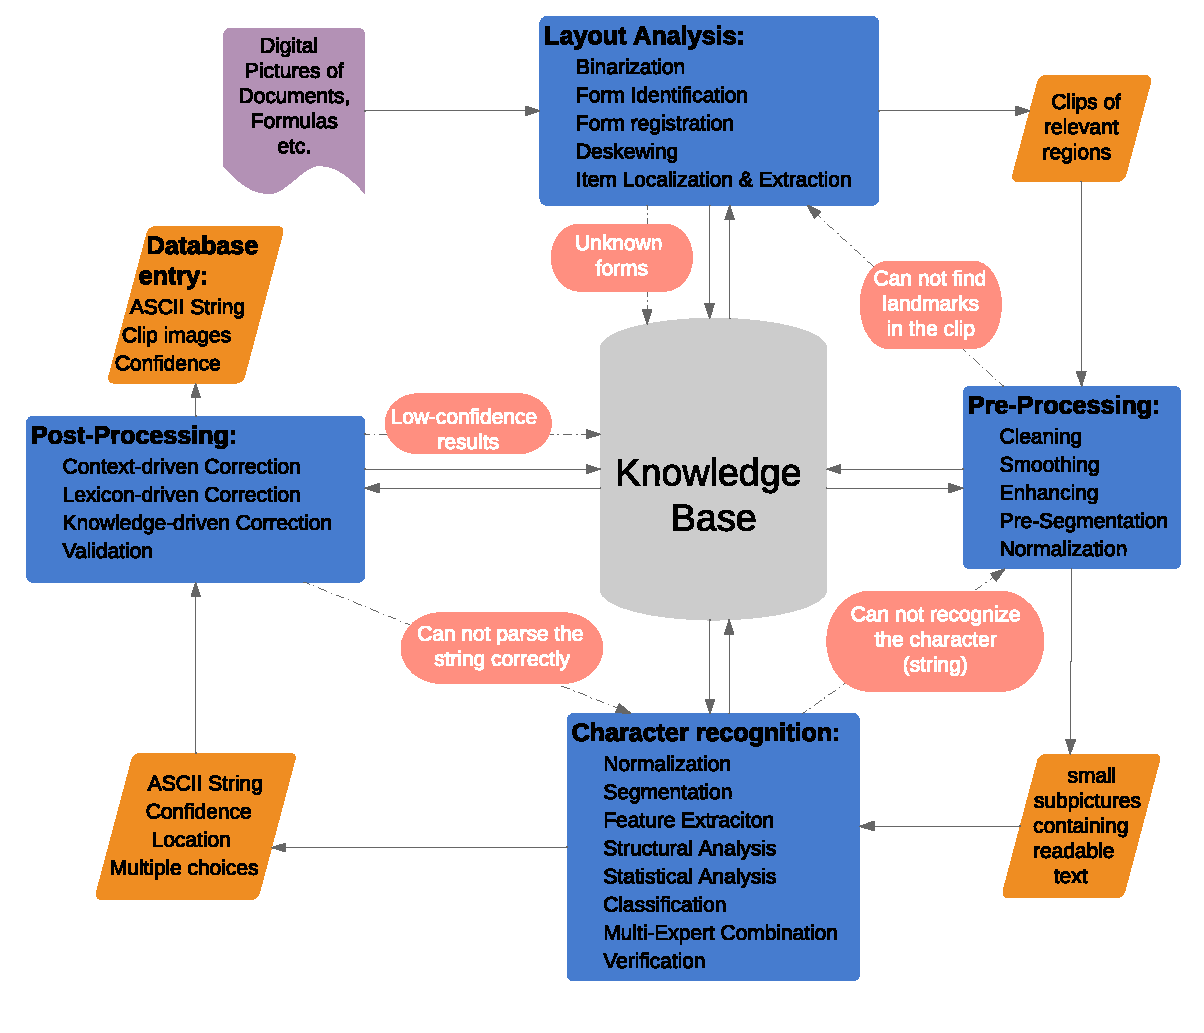
\includegraphics[width=\linewidth]{Ablauf-OCR_Cheriet-et-al.pdf}
			\caption[typisches \gls{ocr}-Ablaufschema]{Schematische Darstellung des 
				Ablaufs in einem intelligenten \gls{ocr}-System (Nachbildung aus 
				\cite[Seite 7]{cher-et-al-ocr})}
			\label{fig:ocr-system}
		\end{figure}
	
		Einen in der heutigen Zeit zentralen Anwendungsfall für die Bildverarbeitung stellt \gls{ocr} dar. Wie der Name bereits vermuten lässt, ist das Ziel der \gls{ocr}, Zeichen oder Formen aus digitalen Bildern zu extrahieren und weiterzuverarbeiten. Schon in den frühen 1950ern - so bei \cite{cher-et-al-ocr} - haben Forscher nach Möglichkeiten gesucht, auf Papier befindlichen Text mit Hilfe von Rechnerkapazitäten einzulesen, um dem Menschen die mühselige Arbeit des manuellen Abtippens von Dokumenten abzunehmen.

		Damit ein System, wie es auf Abbildung \ref{fig:ocr-system} zu 
		erkennen ist, zuverlässig Zeichen erkennen kann, muss es unter 
		anderem auf die Formen der Zeichen trainiert werden und als Input ein für 
		die Anwendung angemessen segmentiertes Bild erhalten. 
		